\documentclass{standalone}
\usepackage{tikz}
\usetikzlibrary{patterns, positioning}


\begin{document}
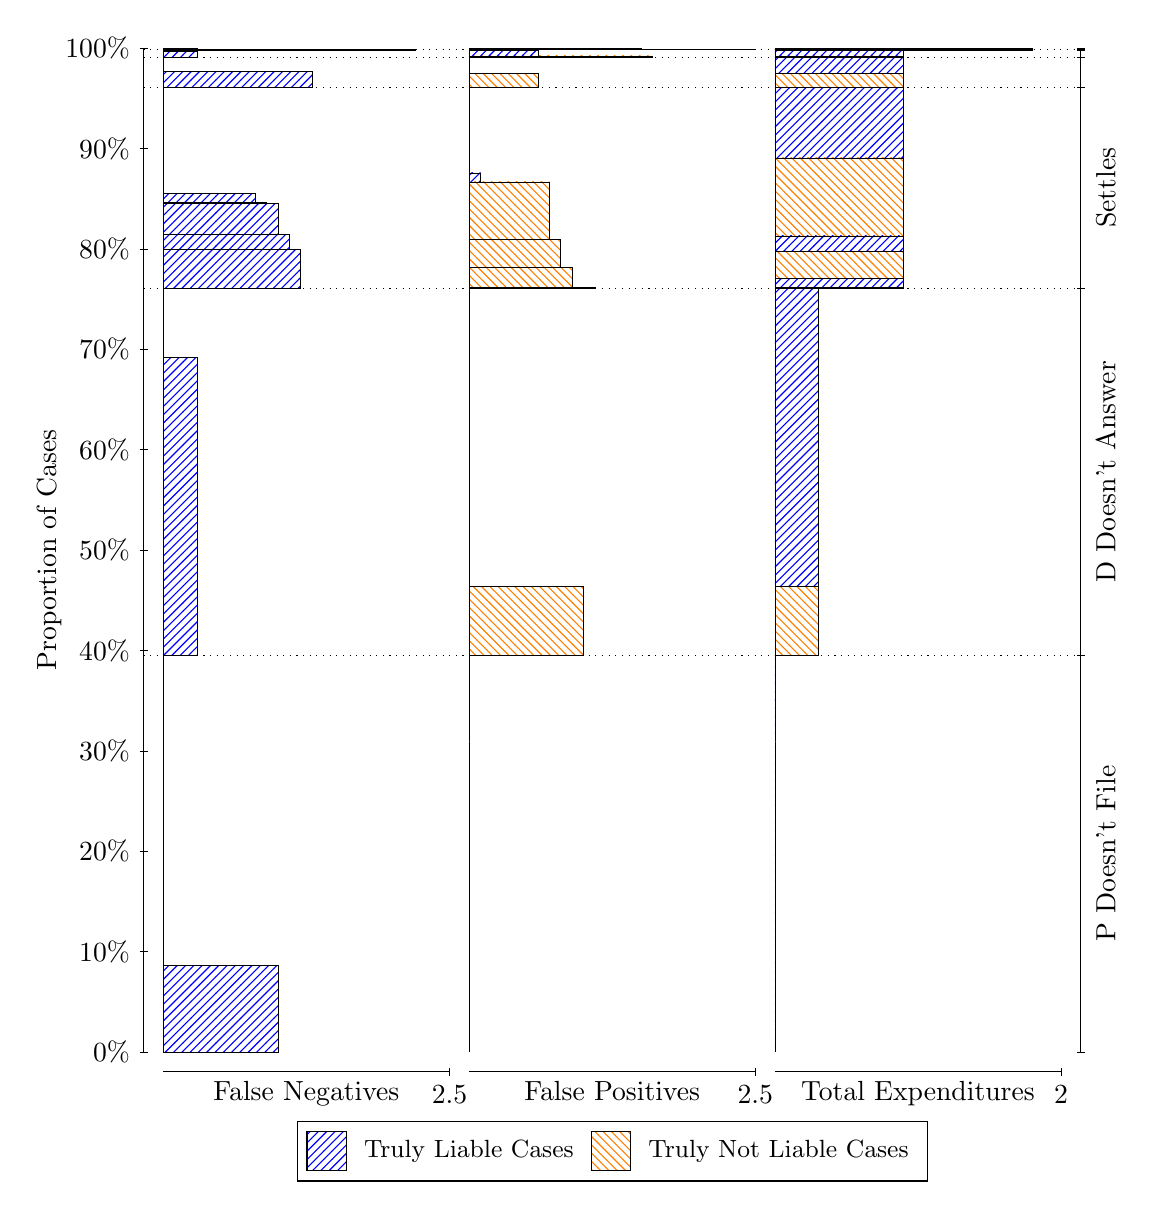
\begin{tikzpicture}
\draw[black, very thin] (1.5,1.75) -- (1.5,14.5);
\node[rotate=90, text=black, anchor=center] at (0.3, 8.125) {Proportion of Cases};
\draw[black, very thin] (1.45,1.75) -- (1.55,1.75);
\node[text=black, anchor=east] at (1.45, 1.75) {0\%};
\draw[black, very thin] (1.45,3.025) -- (1.55,3.025);
\node[text=black, anchor=east] at (1.45, 3.025) {10\%};
\draw[black, very thin] (1.45,4.3) -- (1.55,4.3);
\node[text=black, anchor=east] at (1.45, 4.3) {20\%};
\draw[black, very thin] (1.45,5.575) -- (1.55,5.575);
\node[text=black, anchor=east] at (1.45, 5.575) {30\%};
\draw[black, very thin] (1.45,6.85) -- (1.55,6.85);
\node[text=black, anchor=east] at (1.45, 6.85) {40\%};
\draw[black, very thin] (1.45,8.125) -- (1.55,8.125);
\node[text=black, anchor=east] at (1.45, 8.125) {50\%};
\draw[black, very thin] (1.45,9.4) -- (1.55,9.4);
\node[text=black, anchor=east] at (1.45, 9.4) {60\%};
\draw[black, very thin] (1.45,10.675) -- (1.55,10.675);
\node[text=black, anchor=east] at (1.45, 10.675) {70\%};
\draw[black, very thin] (1.45,11.95) -- (1.55,11.95);
\node[text=black, anchor=east] at (1.45, 11.95) {80\%};
\draw[black, very thin] (1.45,13.225) -- (1.55,13.225);
\node[text=black, anchor=east] at (1.45, 13.225) {90\%};
\draw[black, very thin] (1.45,14.5) -- (1.55,14.5);
\node[text=black, anchor=east] at (1.45, 14.5) {100\%};

\draw[black, very thin] (13.4,1.75) -- (13.4,14.5);
\draw[black, very thin] (13.35,1.75) -- (13.45,1.75);
\node[anchor=west] at (13.35, 1.75) {};
\draw[black, very thin] (13.35,6.7908) -- (13.45,6.7908);
\node[anchor=west] at (13.35, 6.7908) {};
\draw[black, very thin] (13.35,11.446) -- (13.45,11.446);
\node[anchor=west] at (13.35, 11.446) {};
\draw[black, very thin] (13.35,14.003) -- (13.45,14.003);
\node[anchor=west] at (13.35, 14.003) {};
\draw[black, very thin] (13.35,14.379) -- (13.45,14.379);
\node[anchor=west] at (13.35, 14.379) {};
\draw[black, very thin] (13.35,14.477) -- (13.45,14.477);
\node[anchor=west] at (13.35, 14.477) {};
\draw[black, very thin] (13.35,14.484) -- (13.45,14.484);
\node[anchor=west] at (13.35, 14.484) {};
\draw[black, very thin] (13.35,14.5) -- (13.45,14.5);
\node[anchor=west] at (13.35, 14.5) {};

\draw[black, very thin, pattern color=blue, pattern=north east lines] (1.75,1.75) rectangle (3.2033,2.8477);
\draw[black, very thin, pattern color=orange, pattern=north west lines] (1.75,2.8477) rectangle (1.75,6.7908);
\draw[black, very thin, pattern color=blue, pattern=north east lines] (1.75,6.7908) rectangle (2.186,10.572);
\draw[black, very thin, pattern color=orange, pattern=north west lines] (1.75,10.572) rectangle (1.75,11.446);
\draw[black, very thin, pattern color=blue, pattern=north east lines] (1.75,11.446) rectangle (3.494,11.941);
\draw[black, very thin, pattern color=blue, pattern=north east lines] (1.75,11.941) rectangle (3.3487,12.131);
\draw[black, very thin, pattern color=blue, pattern=north east lines] (1.75,12.131) rectangle (3.2033,12.53);
\draw[black, very thin, pattern color=blue, pattern=north east lines] (1.75,12.53) rectangle (3.058,12.535);
\draw[black, very thin, pattern color=blue, pattern=north east lines] (1.75,12.535) rectangle (2.9127,12.651);
\draw[black, very thin, pattern color=orange, pattern=north west lines] (1.75,12.651) rectangle (1.75,14.003);
\draw[black, very thin, pattern color=blue, pattern=north east lines] (1.75,14.003) rectangle (3.6393,14.202);
\draw[black, very thin, pattern color=orange, pattern=north west lines] (1.75,14.202) rectangle (1.75,14.379);
\draw[black, very thin, pattern color=blue, pattern=north east lines] (1.75,14.379) rectangle (2.186,14.455);
\draw[black, very thin, pattern color=orange, pattern=north west lines] (1.75,14.455) rectangle (1.75,14.477);
\draw[black, very thin, pattern color=blue, pattern=north east lines] (1.75,14.477) rectangle (4.9473,14.48);
\draw[black, very thin, pattern color=orange, pattern=north west lines] (1.75,14.48) rectangle (1.75,14.484);
\draw[black, very thin, pattern color=blue, pattern=north east lines] (1.75,14.484) rectangle (2.186,14.497);
\draw[black, very thin, pattern color=orange, pattern=north west lines] (1.75,14.497) rectangle (1.75,14.5);
\draw[black, very thin, pattern color=orange, pattern=north west lines] (5.6333,1.75) rectangle (5.6333,5.6931);
\draw[black, very thin, pattern color=blue, pattern=north east lines] (5.6333,5.6931) rectangle (5.6333,6.7908);
\draw[black, very thin, pattern color=orange, pattern=north west lines] (5.6333,6.7908) rectangle (7.0867,7.6645);
\draw[black, very thin, pattern color=blue, pattern=north east lines] (5.6333,7.6645) rectangle (5.6333,11.446);
\draw[black, very thin, pattern color=orange, pattern=north west lines] (5.6333,11.446) rectangle (7.232,11.46);
\draw[black, very thin, pattern color=orange, pattern=north west lines] (5.6333,11.46) rectangle (7.0867,11.462);
\draw[black, very thin, pattern color=orange, pattern=north west lines] (5.6333,11.462) rectangle (6.9413,11.716);
\draw[black, very thin, pattern color=orange, pattern=north west lines] (5.6333,11.716) rectangle (6.796,12.066);
\draw[black, very thin, pattern color=orange, pattern=north west lines] (5.6333,12.066) rectangle (6.6507,12.799);
\draw[black, very thin, pattern color=blue, pattern=north east lines] (5.6333,12.799) rectangle (5.7787,12.914);
\draw[black, very thin, pattern color=blue, pattern=north east lines] (5.6333,12.914) rectangle (5.6333,14.003);
\draw[black, very thin, pattern color=orange, pattern=north west lines] (5.6333,14.003) rectangle (6.5053,14.18);
\draw[black, very thin, pattern color=blue, pattern=north east lines] (5.6333,14.18) rectangle (5.6333,14.379);
\draw[black, very thin, pattern color=orange, pattern=north west lines] (5.6333,14.379) rectangle (7.9587,14.401);
\draw[black, very thin, pattern color=blue, pattern=north east lines] (5.6333,14.401) rectangle (6.5053,14.477);
\draw[black, very thin, pattern color=orange, pattern=north west lines] (5.6333,14.477) rectangle (6.5053,14.481);
\draw[black, very thin, pattern color=blue, pattern=north east lines] (5.6333,14.481) rectangle (5.6333,14.484);
\draw[black, very thin, pattern color=orange, pattern=north west lines] (5.6333,14.484) rectangle (9.2667,14.487);
\draw[black, very thin, pattern color=blue, pattern=north east lines] (5.6333,14.487) rectangle (7.8133,14.5);
\draw[black, very thin, pattern color=orange, pattern=north west lines] (9.5167,1.75) rectangle (9.5167,5.6931);
\draw[black, very thin, pattern color=blue, pattern=north east lines] (9.5167,5.6931) rectangle (9.5167,6.7908);
\draw[black, very thin, pattern color=orange, pattern=north west lines] (9.5167,6.7908) rectangle (10.062,7.6645);
\draw[black, very thin, pattern color=blue, pattern=north east lines] (9.5167,7.6645) rectangle (10.062,11.446);
\draw[black, very thin, pattern color=orange, pattern=north west lines] (9.5167,11.446) rectangle (11.152,11.46);
\draw[black, very thin, pattern color=blue, pattern=north east lines] (9.5167,11.46) rectangle (11.152,11.576);
\draw[black, very thin, pattern color=orange, pattern=north west lines] (9.5167,11.576) rectangle (11.152,11.925);
\draw[black, very thin, pattern color=blue, pattern=north east lines] (9.5167,11.925) rectangle (11.152,12.115);
\draw[black, very thin, pattern color=orange, pattern=north west lines] (9.5167,12.115) rectangle (11.152,13.104);
\draw[black, very thin, pattern color=blue, pattern=north east lines] (9.5167,13.104) rectangle (11.152,14.003);
\draw[black, very thin, pattern color=orange, pattern=north west lines] (9.5167,14.003) rectangle (11.152,14.18);
\draw[black, very thin, pattern color=blue, pattern=north east lines] (9.5167,14.18) rectangle (11.152,14.379);
\draw[black, very thin, pattern color=orange, pattern=north west lines] (9.5167,14.379) rectangle (11.152,14.401);
\draw[black, very thin, pattern color=blue, pattern=north east lines] (9.5167,14.401) rectangle (11.152,14.477);
\draw[black, very thin, pattern color=orange, pattern=north west lines] (9.5167,14.477) rectangle (12.787,14.481);
\draw[black, very thin, pattern color=blue, pattern=north east lines] (9.5167,14.481) rectangle (12.787,14.484);
\draw[black, very thin, pattern color=orange, pattern=north west lines] (9.5167,14.484) rectangle (12.787,14.487);
\draw[black, very thin, pattern color=blue, pattern=north east lines] (9.5167,14.487) rectangle (12.787,14.5);
\draw[black, dotted] (1.5,6.7908) -- (13.4,6.7908);
\draw[black, dotted] (1.5,11.446) -- (13.4,11.446);
\draw[black, dotted] (1.5,14.003) -- (13.4,14.003);
\draw[black, dotted] (1.5,14.379) -- (13.4,14.379);
\draw[black, dotted] (1.5,14.477) -- (13.4,14.477);
\draw[black, dotted] (1.5,14.484) -- (13.4,14.484);
\draw[black, very thin] (1.75,1.5) -- (5.3833,1.5);
\node[text=black, anchor=north] at (3.5667, 1.5) {False Negatives};
\draw[black, very thin] (5.3833,1.45) -- (5.3833,1.55);
\node[text=black, anchor=north] at (5.3833, 1.45) {2.5};

\draw[black, very thin] (5.6333,1.5) -- (9.2667,1.5);
\node[text=black, anchor=north] at (7.45, 1.5) {False Positives};
\draw[black, very thin] (9.2667,1.45) -- (9.2667,1.55);
\node[text=black, anchor=north] at (9.2667, 1.45) {2.5};

\draw[black, very thin] (9.5167,1.5) -- (13.15,1.5);
\node[text=black, anchor=north] at (11.333, 1.5) {Total Expenditures};
\draw[black, very thin] (13.15,1.45) -- (13.15,1.55);
\node[text=black, anchor=north] at (13.15, 1.45) {2};

\node[text=black, centered, rotate=90] at (13.72, 4.2704) {P Doesn't File};
\node[text=black, centered, rotate=90] at (13.72, 9.1184) {D Doesn't Answer};
\node[text=black, centered, rotate=90] at (13.72, 12.725) {Settles};





\draw (7.449999999999999,1.5) node[draw=none] (baseCoordinate) {};
\begin{scope}[align=center]
        \matrix[scale=0.5, draw=black, below=0.5cm of baseCoordinate, nodes={draw}, column sep=0.1cm]{
            \node[rectangle, draw, minimum width=0.5cm, minimum height=0.5cm, pattern color=blue, pattern=north east lines] {}; &
            \node[draw=none, font=\small, text=black] (B) {Truly Liable Cases}; &
            \node[rectangle, draw, minimum width=0.5cm, minimum height=0.5cm, pattern color=orange, pattern=north west lines] {}; &
            \node[draw=none, font=\small, text=black] (B) {Truly Not Liable Cases}; \\
            };
\end{scope}

\end{tikzpicture}
\end{document}